\subsection{Convergence}
\begin{figure}[t]
\center
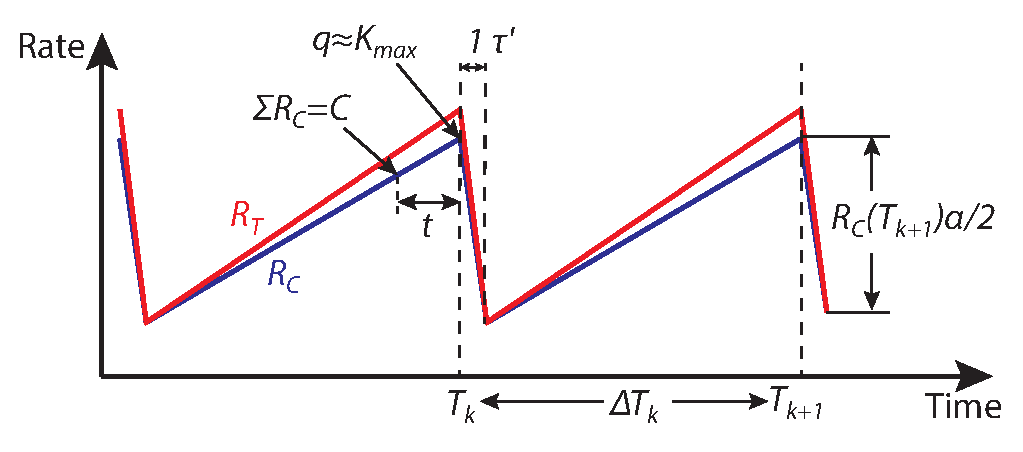
\includegraphics[width=0.4\textwidth]{figures/dcqcn_convergence.eps}
\caption{DCQCN flow rate update.}
\label{fig:dcqcn_convergence}
\end{figure}

In Section~\ref{sec:dcqcn_stability}, we showed that for reasonable parameter
settings,  DCQCN is stable {\em after} flows converge to the unique fixed point.
We also showed that at the fixed point, the flows share the bandwidth equally.
However, two questions remain unanswered: $(i)$ do flows the always converge
to this fixed point, and $(ii)$ how fast do flows converge? 

We cannot answer these questions using the fluid model, so we construct and
analyze a discrete model of the rate adjustment at the RP. The default parameter
settings given in~\cite{dcqcn} set both the Timer $T$ and $\alpha$ update
interval $\tau '$ equal to $55\mu s$. Thus, we use $\tau '$ as the unit of time.
The process of DCQCN rate update is similar to TCP AIMD, as shown in
Figure~\ref{fig:dcqcn_convergence}.  The flows get the peak rates at $T_k$. For
simplicity, we assume all flows get to the peak at the same time, which is
likely to happen because the queue peak at the bottleneck leads to high marking
probability for all flows. When the flow gets ECN marks at $T_k$, it reduces its
rate in one unit of time, then starts multiple consecutive additive rate
increases on $R_T^{(i)}$:\footnote{For simplicity, we omit hyper-increase and set 
$R_T = R_C$ upon rate decrease. This is a simplified version of QCN.}

\begin{equation}
\small
R_T^{(i)}({T_{k + 1}}) = \left( {1 - \frac{{{\alpha ^{(i)}}({T_k})}}{2}} \right)R_C^{(i)}({T_k}) + \left( {\Delta {T_k} - 1} \right){R_{AI}}
\label{eq:converge_rc}
\end{equation}
where $\Delta {T_k} \buildrel \Delta \over = {T_{k + 1}} - {T_k}$. During the consecutive 
additive rate increase, {\em i.e.,} $\forall t \in ({T_k} + 1,{T_{k + 1}}]$, $R_C^{(i)}$ and $R_T^{(i)}$ 
have following relationship according to DCQCN's definition:
\begin{equation}
\small
R_C^{(i)}(t + 1) = \frac{1}{2}\left( {R_C^{(i)}(t) + R_T^{(i)}(t + 1)} \right)\\
\label{ref:discrete_rc}
\end{equation}
\begin{equation}
\small
R_T^{(i)}(t + 1) = R_T^{(i)}(t) + {R_{AI}}
\label{ref:discrete_rt}
\end{equation}

By (\ref{ref:discrete_rc})-$\frac{1}{2}\times$(\ref{ref:discrete_rt}), we get:

\begin{equation}
\small
\begin{array}{l}
R_C^{(i)}(T_{k + 1}) - R_T^{(i)}(T_{k + 1}) + {R_{AI}}\\
 = \frac{1}{2}\left( {R_C^{(i)}(T_{k + 1} - 1) - R_T^{(i)}(T_{k + 1} - 1) + {R_{AI}}} \right)\\
 = ... = {\left( {\frac{1}{2}} \right)^{\Delta {T_k}-1}}\left( {R_C^{(i)}({T_k} + 1) - R_T^{(i)}({T_k} + 1) + {R_{AI}}} \right)
\end{array}
\end{equation}

From this, we know that during a consecutive additive rate increase phase, $R_T^{(i)} - R_C^{(i)}$
will converge towards $R_{AI}$ exponentially. In common cases, the step of additive increase,
$\Delta {T_k} - 1$, is around 10 or even more\footnote{This can be easily estimated by numerical approaches, 
thus omitted for brevity}. 
%Also, due to DCQCN definition, we have $R_C^{(i)}({T_k} + 1) = R_T^{(i)}({T_k} + 1)$
%as shown in Figure~\ref{fig:dcqcn_convergence}. 
Therefore, we can safely approximate $R_T^{(i)}$ by:
\begin{equation}
\small
R_T^{(i)}({T_k}) \approx R_C^{(i)}({T_k}) + {R_{AI}},\forall k = 1,2,...
\end{equation}
Back to Equation~\ref{eq:converge_rc}, we must further know $\alpha ^{(i)}({T_k})$ and $\Delta T_k$ to 
analyze $R_C(T_k)$. During $\Delta T_k$, $\alpha ^{(i)}({T_k})$ has one increase event as Equation~\ref{eq:rp_dec},
followed by $\Delta T_k - 1$ recover events as Equation~\ref{eq:rp_alpha_recover}:
\begin{equation}
\small
{\alpha ^{(i)}}({T_{k + 1}}) = {(1 - g)^{\Delta {T_k} - 1}}\left( {(1 - g){\alpha ^{(i)}}({T_k}) + g} \right)
\label{eq:converge_alpha}
\end{equation}
For another flow, {\em e.g.,} the $j$th flow, we can simply rewrite above equation by replacing 
$(i)$ with $(j)$. We subtract the equation of $j$th flow from the equation of $i$th flow, we get:
\begin{equation}
\small
\begin{array}{l}
{\alpha ^{(i)}}({T_{k + 1}}) - {\alpha ^{(j)}}({T_{k + 1}}) = {(1 - g)^{\Delta {T_k}}}\left( {{\alpha ^{(i)}}({T_k}) - {\alpha ^{(j)}}({T_k})} \right)\\
 = ... = {(1 - g)^{\sum\nolimits_{l = 0}^k {\Delta {T_l}} }}\left( {{\alpha ^{(i)}}({T_0}) - {\alpha ^{(j)}}({T_0})} \right)
\end{array}
\label{eq:converge_alphaarray}
\end{equation}
This tells us the difference of $\alpha^{(i)}$ of different flows will quickly decrease exponentially. So $\alpha^{(i)}$
of different flows will converge to the same value, and the converging speed is determined by $g$ and
$\Delta T_k$. 

Once the $\alpha$ of different flows converge to the same value $\alpha(T_{k'})$ at some $T_{k'}$, we can show 
the rates $R_C$ converge afterwards. We rewrite the $j$th flow's Equation~\ref{eq:converge_rc}, and subtract it 
from Equation~\ref{eq:converge_rc}, we get:
\begin{equation}
\small
\begin{array}{l}
R_C^{(i)}({T_{k + 1}}) - R_C^{(j)}({T_{k + 1}}) = \left( {1 - \frac{{\alpha ({T_k})}}{2}} \right)\left( {R_C^{(i)}({T_k}) - R_C^{(j)}({T_k})} \right)\\
 = ... = \prod\limits_{l = k'}^k {\left( {1 - \frac{{\alpha ({T_l})}}{2}} \right)} \left( {R_C^{(i)}({T_{k'}}) - R_C^{(j)}({T_{k'}})} \right)
\end{array}
\label{eq:converge}
\end{equation}
As long as $\alpha ({T_k})$ has a lower bound that is greater than 0, the rates $R_C$ of different flows 
converge exponentially. In Appendix~\ref{sec:alpha_proof}, we prove that:
\begin{equation}
\small
\alpha ({T_0}) > ... > \alpha ({T_k}) > \alpha ({T_{k + 1}}) > ... > {\alpha ^*} > 0
\label{eq:converge_alphastar}
\end{equation}
where $\alpha^{*}$ is the fixed point of the $\alpha$ array (Equation~\ref{eq:converge_alpha}),
which is the solution of the following equation\footnote{${\Delta {T^*}}$ can be described by 
$\alpha^{*}$ and DCQCN parameters, as shown in Appendix.}:
\begin{equation}
\small
{\alpha ^*} = {(1 - g)^{\Delta {T^*}}}\left( {(1 - g){\alpha ^*} + g} \right)
\end{equation}
Equation~\ref{eq:converge_alphastar} concludes our proof. Combining Equation~\ref{eq:converge_rc}, 
we know that $R_C$ is converging at the rate of at least $( {1 - \frac{{{\alpha ^{*}}}}{2}} )^k$, 
$k$ is the number of AIMD cycles.

\begin{figure}[t]
\center
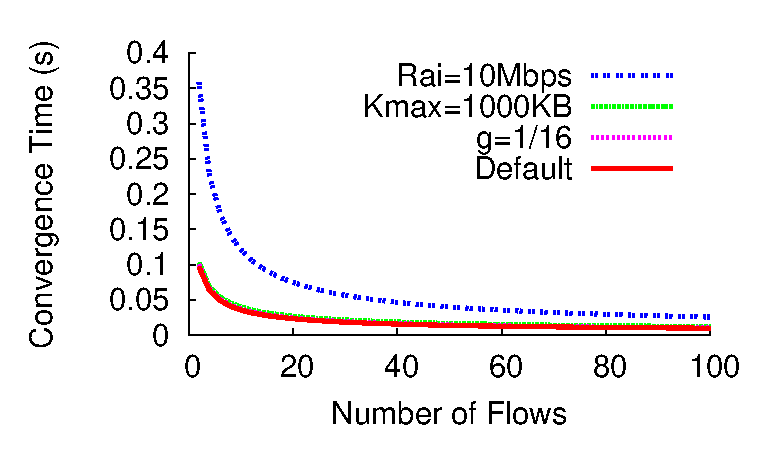
\includegraphics[width=0.4\textwidth]{figures/dcqcn_convergence_time.eps}
\caption{Upper bound on DCQCN convergence time under conservative assumptions}
\label{fig:dcqcn_convergence_time}
\end{figure}

\begin{figure}[t]
\center
\subfigure[]
{
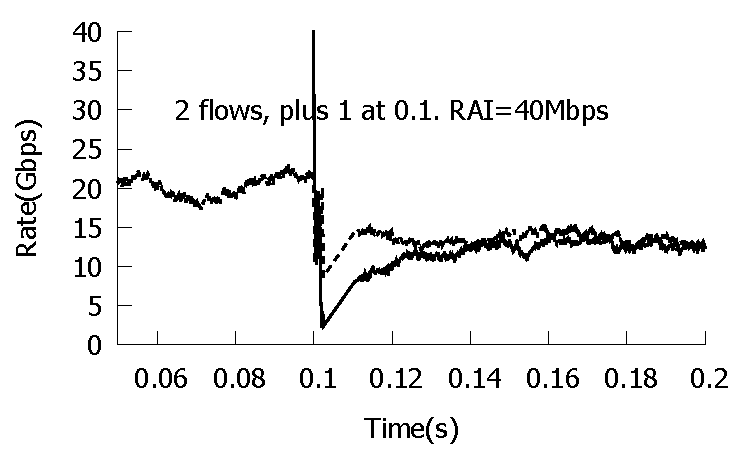
\includegraphics[width=0.35\textwidth]{figures/dcqcn_converge_3.pdf}
\label{fig:dcqcn_convergence_sim_3}
}
\subfigure[]
{
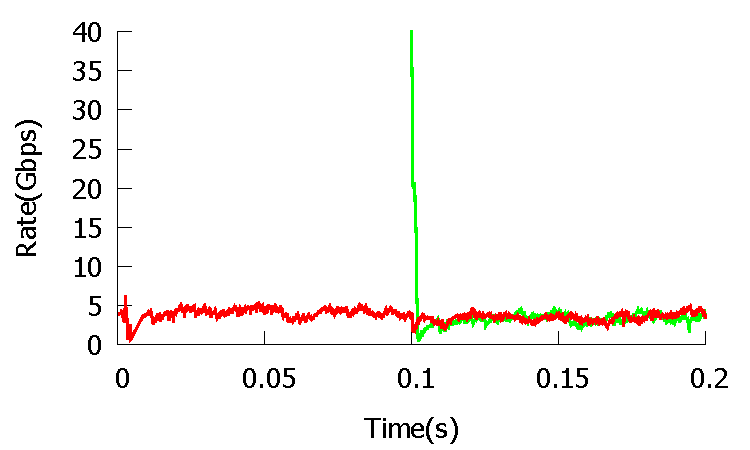
\includegraphics[width=0.35\textwidth]{figures/dcqcn_converge_11.pdf}
\label{fig:dcqcn_convergence_sim_11}
}
\subfigure[]
{
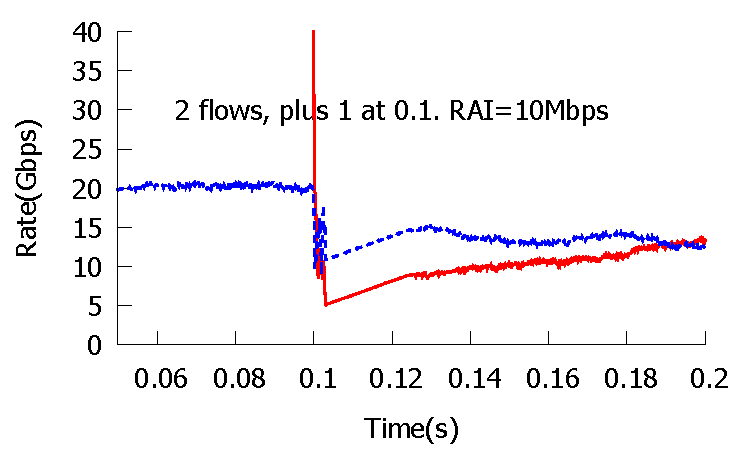
\includegraphics[width=0.35\textwidth]{figures/dcqcn_converge_3rai.pdf}
\label{fig:dcqcn_convergence_sim_3rai}
}
\caption{DCQCN convergence: simulation results}
\label{fig:dcqcn_convergence_sim}
\end{figure}

\para{Convergence time.} 
In the above analysis, the convergence has two phases: (1) $\alpha ^{(i)}$
converge to the same value (not necessarily at $\alpha^*$); (2) $R_C^{(i)}$
converge along with $\alpha \to \alpha^*$.  In practice, the flows that
encounter congestion for the first time all have the same initial value of 1.
Therefore, we mainly focus on the second phase. We define the system as having
``converged'' when the difference of any two flows is no more than 10\% of
expected fair share.

We now derive an upper bound convergence time of under several worst-case
assumptions. First, we assume that the value of $\alpha ({T_k})$ is $\alpha ^*$.
In practice, $\alpha ({T_k}) > \alpha ^*$, so the flows will converge faster
than our estimation, given the term $(1 - \alpha /2)^T$ in
Equation~\ref{eq:converge}.  Second, we assume that the switch does not mark ECN
until the queue length hits $K_{max}$, opposed to using RED. 

The maximum possible difference between initial rates of two flows can at most
be $C$. So, an upper bound on the convergence time is the time required for this
difference to fall from $C$ to less than $\frac{0.1 \times C}{N}$. This is
simply the smallest value of $x$ that satisfies the following inequality: 

\begin{equation} 
\small 
{ \left( {1 - \frac{{{\alpha ^*}}}{2}} \right)^{\frac{x}{{\tau '\Delta{T^*}}}}}C \le \frac{0.1 \times C}{N} 
\end{equation}

We solve equation numerically for different parameter settings. The results are
shown Figure~\ref{fig:dcqcn_convergence_time}. With default parameter settings,
DCQCN converges within 100ms, and the convergenced time decreases quickly as the
number of flow increases.  We have also calculated convergence time for a range
of different values of $R_{AI}$, $K_{max}$ and $g$. Sample results are shown in
Figure~\ref{fig:dcqcn_convergence_time}. We found that convergence time is
determined primarily $R_{AI}$, which is not surprising.

We have verified these results with packet simulations. Sample results are shown
in Figure~\ref{fig:dcqcn_convergence_sim}. In
Figure~\ref{fig:dcqcn_convergence_sim_3}, we start two flows at 40Gbps, and let
them stabilize. They stabilize to roughly 20Gbps, as expected. Then, at time
0.1, we start the third flow, at 40Gbps. As we see, the three flows converge to
13Gbps in well within 100ms. Figure~\ref{fig:dcqcn_convergence_sim_3rai} shows
similar results, except that we use a lower value of $R_{AI}$. As expected, it
takes longer for the flows to converge. In
Figure~\ref{fig:dcqcn_convergence_sim_11} we start with 10 flows, and add an
11th flow at time 0.1. The convergecne time is lower as the the number of flows
is higher.


%Note that Figure~\ref{fig:dcqcn_converge_time}
%is the upper bound of convergence time with conservative assumptions. 






